\documentclass[a4paper,11pt]{article}

\usepackage[latin1]{inputenc}
\usepackage[T1]{fontenc}
\usepackage{bbm} %math chars
\usepackage{amsmath}
\usepackage{indentfirst}
\usepackage{fullpage} %minimizes the default margins
\usepackage{url}
\usepackage{graphicx}
\usepackage[center,footnotesize]{caption} %options des legendes des graphes
\usepackage[section]{placeins} %place les figures d'une section avant le debut de la suivante
\usepackage{subfig} %a) b) c)

\title{Exercises - Week 6}
\date{}
\author{Genomics and bioinformatics}

\begin{document}
\maketitle

This series is about phylogenetic trees and a complement to HMMs.

\section{Phylogenetic trees}

Circadian rhythms (often referred to as the ``body clock``) are
ubiquitous in most life forms. The ``period`` family of genes is an 
essential component of this clock.

The table below provides BLAST scores of pairwise
alignments for six period family proteins from three different
species, 

\begin{enumerate}
\item {\bf dm\_per} from {\it Drosophila melanogaster}, i.e. fruit fly,
\item {\bf dr\_per2} and {\bf dr\_per3} from {\it Danio rerio}, i.e. zebra fish,
\item {\bf mm\_per1}, {\bf mm\_per2} and {\bf mm\_per3} from {\it Mus
  musculus}, i.e. mouse.
\end{enumerate}

\begin{center}
	\begin{tabular} {| l || l | l | l | l | l | l |}
	\hline
 	& dm\_per & dr\_per2 & dr\_per3 & mm\_per1 & mm\_per2 & mm\_per3 \\ \hline\hline
	dm\_per & -  & 116 & 125 & 129 & 123 & 121 \\	\hline
	dr\_per2 &	114 & - & 661 & 887 & 947& 497 \\	\hline
	dr\_per3 & 123 & 644 & - & 667 & 666 & 699 \\	\hline
	mm\_per1 & 126 & 745 & 572 & - & 640 & 80 \\	\hline
	mm\_per2 & 126 & 984 & 680 & 832 & - & 455 \\	\hline
	mm\_per3 & 124 & 499 & 709 & 537 & 488 & - \\
	\hline
	\end{tabular}
\end{center}
\vspace{0.05 cm}

\begin{enumerate}
\item Based on the table above, draw the gene tree for the six period
  proteins (dm\_per, dr\_per2, dr\_per3,  mm\_per1, mm\_per2,
  mm\_per3). 
\item Using this tree, give examples of:
  \begin{itemize} 
  \item an orthologous pair, 
  \item a paralogous pair in the same species, and 
  \item a paralogous pair in different species.
  \end{itemize}
\end{enumerate}

\section{Another HMM}

\subsection{The Viterbi algorithm}

In series 4, you designed a Hidden Markov Model. We shall now use this model to actually find the GC-rich isochore region. However, for computational reasons, the genome and GC-rich region lengths are set to 100 and 10, respectively, leading to $p=1/10$ and $q=1/90$. We have also included a starting state $S$. See the figure below.


\begin{center}
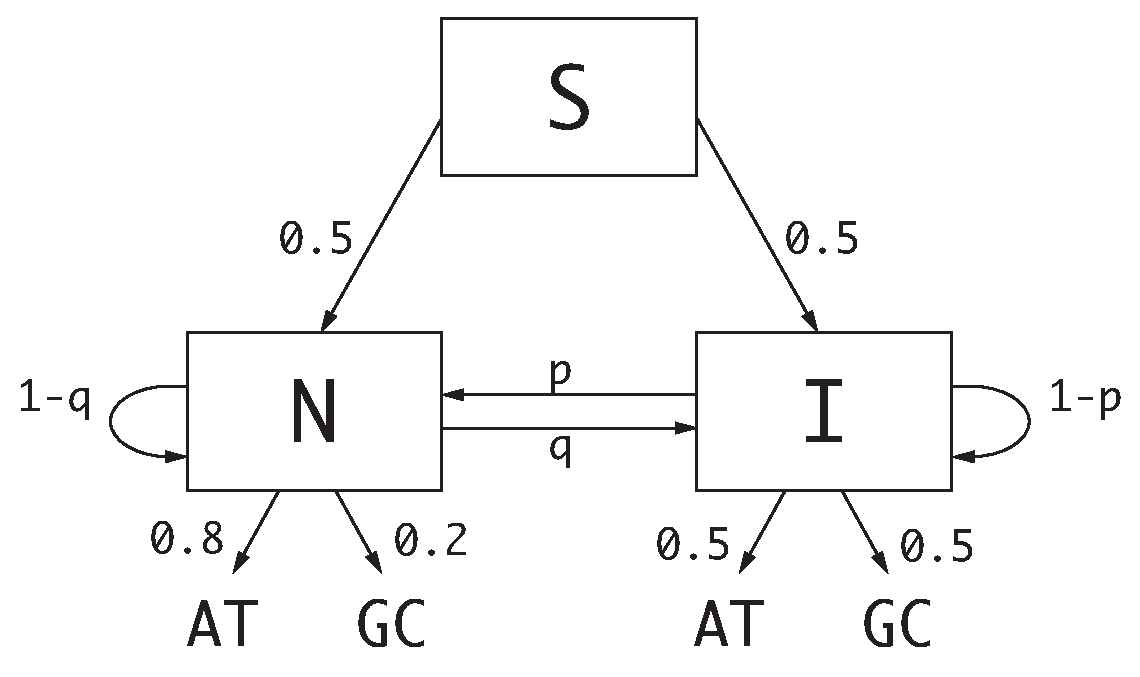
\includegraphics[width=0.7\textwidth]{fig1.eps}\\
\vspace{0.5cm}
{\bf The Hidden Markov Model}
\end{center}

In the course, you have seen the Viterbi algorithm based on the following scoring function:

$$
F_{n,s} = E(T_n, s) \cdot \max_{\sigma \in \{S, N, I\}}\left\{F_{n-1, \sigma} \cdot M(\sigma, s)  \right\}~, \ n = 1, 2, \dots
$$
The initial condition is $F_{0, \sigma} = 1$ if $\sigma = S$ and $F_{0, \sigma} = 0$ otherwise. Use this formula to fill in the following table by hand and then use backtracking to find the most probable hidden state sequence associated to the observed sequence "ATC":

\begin{center}
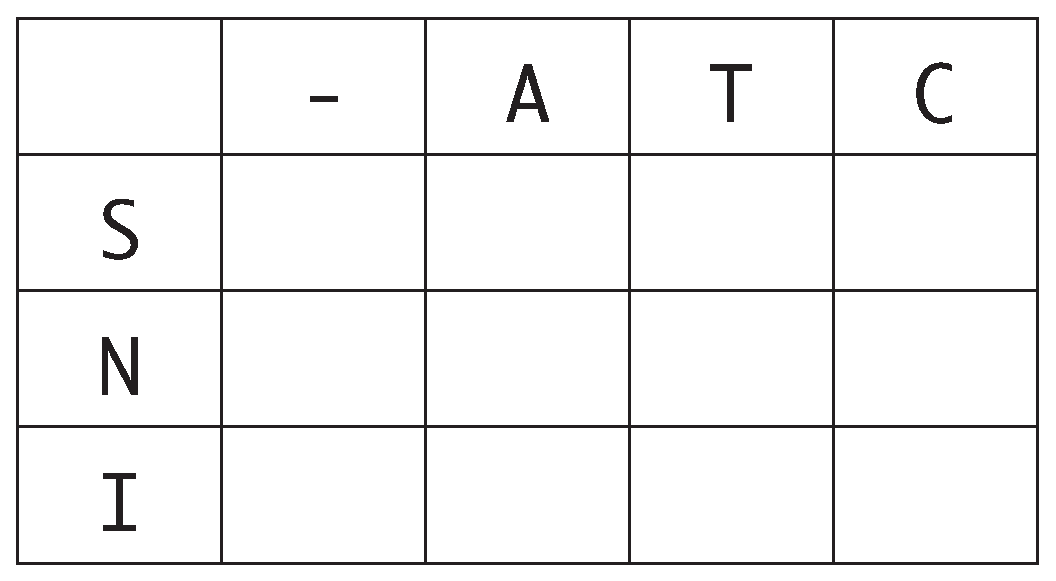
\includegraphics[width=0.7\textwidth]{fig2.eps}\\
\vspace{0.5cm}
{\bf The Table}
\end{center}

\newpage

\subsection{Using R}

In this exercise, we show you how to use an existing package to model a problem with an HMM and solve it. There exist such packages for most programming languages, but here we arbitrarily chose R.

\subsubsection{Get started}

Start R, then download, install and import the HMM package:

\begin{verbatim}
install.packages("HMM")
library(HMM)
\end{verbatim}

Create an vector \texttt{states} of hidden states, an vector \texttt{emissions} of emission, a vector \texttt{initProb} with the probabilities of the initial state, a matrix \texttt{transProb} with the transition probabilities, a matrix \texttt{emissionProb} 
with the emission probabilities:

\begin{verbatim}
states <- c("S","N","I")
emissions <- c("C","G","A","T","-")
initProb <- c(1,0,0)
transProb <- matrix(c(0,0,0,1/2,89/90,0.1,1/2,1/90,0.9), 3)
emissionProb <- matrix(c(0,0.1,0.25,0,0.1,0.25,0,0.4,0.25,0,0.4,0.25,1,0,0), 3)
\end{verbatim}

Create the model with these parameters:

\begin{verbatim}
hmm <- initHMM(states, emissions, initProb, transProb, emissionProb)
hmm  # prints a summary of the model
\end{verbatim}

Using the model created above, generate random observations of length 100:
\begin{verbatim}
simulation <- simHMM(hmm,101)
simulation  # prints the chosen hidden states and emissions sequences
\end{verbatim}

\subsubsection{Visualize}\label{plot}

Copy and paste the following code to visualize the situation. The plot on the top shows the observed sequence,
the one at the bottom shown the hidden states:

\begin{verbatim}
obsToVal <- function(obs){
	if((obs == "A") | (obs=="T")){return(2)}
	else {return(4)}
}
stateToVal <- function(st){
	if(st == "N"){return (1)}
	if(st == "I"){return (3)}
	else {return ("NA")}
}
l_states=length(simulation$states); l_obs=length(simulation$observation) 
par(mfrow=c(2,1))
plot(sapply(simulation$observation[2:l_obs], obsToVal),pch=19,ylim=c(0,8),
col=sapply(simulation$observation[2:l_obs], obsToVal),cex=.5)
legend("topright",c("A/T","G/C"),pch=19,col=c("red","blue"))
plot( sapply(simulation$states[2:l_states], stateToVal),type="l",ylim=c(0,5))
\end{verbatim}

\subsubsection{Forward, Backward algorithms}

Here are the commands to run the forward and backward algorithms. What is the probability of the observed sequence, given the model ? 

\begin{verbatim}
logForwardProb <- forward(hmm, simulation$observation)
exp(logForwardProb)
logBackwardProb <- backward(hmm, simulation$observation)
exp(logBackwardProb)
\end{verbatim}

\noindent \textit{Indication:} For an observed sequence (without the symbol "-") of length N, the probability is given by the sum of three probabilities at time t=N+1 in the forward case, and the sum of the probabilities weighed by the initial state $\pi = (1,0,0)$ at time t=1 in the backward case. 

\subsubsection{Viterbi}

The function \texttt{simHMM} returns a path of (hidden) states and associated observations. Suppose now that  we have an observed sequence and that we want to compute the corresponding most probable sequence of hidden states. Try first to guess where are the ``I'' region(s) are in the following sequence:

\begin{verbatim}
observation <- c("-","A", "T", "A", "A", "A", "A", "T", "A", "A", "T", "T", "T", "T", "T",
 "A", "T", "A", "A", "C", "T", "A", "T", "A", "T", "A", "T", "G", "T", "A", "C", "A", 
 "T", "A", "T", "T", "T", "T", "T", "A", "T", "T", "A", "A", "T", "T", "A", "G", "C", 
 "G", "C", "T", "T", "C", "C", "G", "A", "A", "C", "T", "A", "G", "G", "A", "G", "A", 
 "G", "C", "G", "T", "T", "T", "A", "T", "T", "T", "T", "T", "T", "T", "T", "A", "T", 
 "T", "T", "A", "A", "A", "A", "T", "A", "T", "A", "C", "T", "T", "A", "A", "A", "A", "A")
\end{verbatim}

Now we are going to find the most probable hidden sequence that explains these observations thanks to the Viterbi algorithm. Is it close to what you expected ? 

\begin{verbatim}
viterbi <- viterbi(hmm, observation)
viterbi
\end{verbatim}
To visualize the sequences, you may use the plot functions used in point \ref{plot}. 

\subsubsection{Baum-Welsch}

Finally, let us admit that our transition and emission probabilities are just a first guess, but we would like to update the model parameters by training it with the Baum-Welsch algorithm:

\begin{verbatim}
bw = baumWelch(hmm, observation, 10)  # 10 iterations
print(bw$hmm)
\end{verbatim}

\end{document}











